\section{Detecci�n de ves�culas}

\subsection{Espacio de color}
\begin{frame}
	\frametitle{Espacio de color}
	�C�mo representamos los colores y la luz en el ordenador?
	\begin{itemize}
		\item Espacios de color posibles
		\item Luminancia vs Crominancia
		\item YUV vs L*a*b
	\end{itemize}
	Luminancia: detecci�n de bordes\\
	Crominancia: detecci�n de piel y falsos positivos
\end{frame}

\begin{frame}
	\frametitle{Luminancia vs Crominancia}
	\begin{tabular}{cc}
		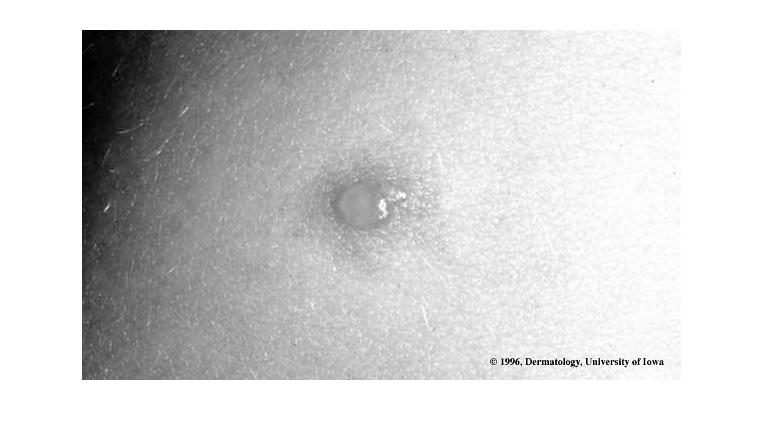
\includegraphics[width=2in]{Resources/CompL-Varicel-02.jpg} & Luminancia - componente L \\
	\end{tabular}
\end{frame}

\begin{frame}
	\frametitle{Luminancia vs Crominancia}
	\begin{tabular}{cc}
		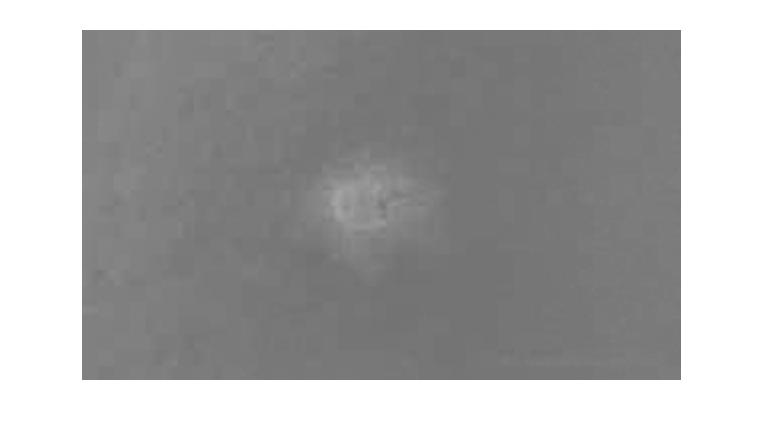
\includegraphics[width=2in]{Resources/CompA-Varicel-02.jpg} & Crominancia - componente a \\
	\end{tabular}
\end{frame}

\begin{frame}
	\frametitle{Luminancia vs Crominancia}
	\begin{tabular}{cc}
		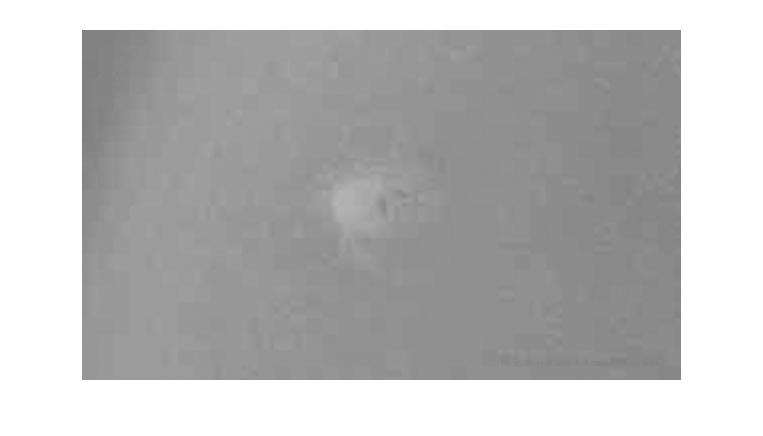
\includegraphics[width=2in]{Resources/CompB-Varicel-02.jpg} & Crominancia - componente b \\
	\end{tabular}
\end{frame}

\subsection{Detecci�n de bordes}
\begin{frame}
	\frametitle{Detecci�n de bordes}
	\begin{itemize}
		\item Resulta sencillo para el ser humano
		\item Borde: frontera entre el objeto y el fondo
		\item Existen varios m�todos (Canny, Roberts, Sobel o Prewitt)
		\item Objetivos de un detector de borde:
		\begin{itemize}
			\item Baja tasa de error
			\item Buena localizaci�n del borde
		\end{itemize}
	\end{itemize}
\end{frame}

\begin{frame}
	\frametitle{M�todo de Canny}
	\begin{itemize}
		\item Robusto contra el ruido
		\item Gran adaptabilidad
		\item Etapas del m�todo:
		\begin{itemize}
			\item Suavizado de la imagen: Filtro gaussiano\\
			\item Obtenci�n del gradiente: Filtro pasa altos en direcci�n vertical y horizontal \\
			\item Supresi�n de puntos que no son m�ximos locales: Adelgazamiento del ancho de los bordes hasta lograr bordes de un p�xel de ancho\\
			\item Umbral con hist�resis: Funci�n de hist�resis basada en dos umbrales; con este proceso se trata de reducir la posibilidad de aparici�n de contornos falsos.\\
		\end{itemize}
	\end{itemize}
\end{frame}

\begin{frame}
	\frametitle{Operaciones morfol�gicas}
	\begin{itemize}
		\item Herramientas muy utilizadas en el procesamiento de im�genes
		\item Simplificar los datos de una imagen
		\item Preservar las caracter�sticas esenciales
		\item Eliminar aspectos irrelevantes
		\item bridge: Une pixeles que est�n separados
		\item Otras operaciones: open, close, clean
	\end{itemize}
\end{frame}

\begin{frame}
	\frametitle{Ejemplo: Bordes detectados en algunas im�genes}
	\begin{columns}[c]
	\column{1.5in}
		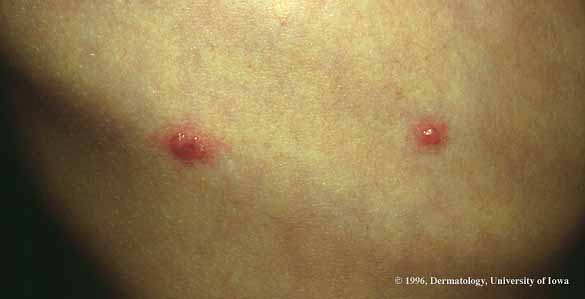
\includegraphics[scale=2.33]{Resources/Varicel-03.jpg} \\
		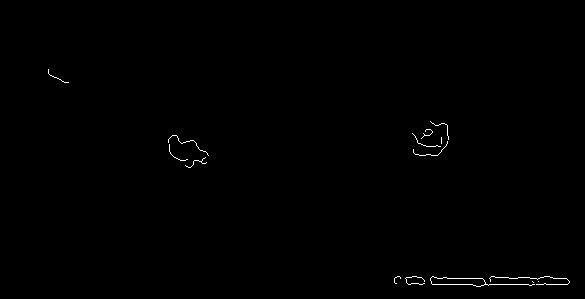
\includegraphics[scale=0.21]{Resources/Varicel-03_bordes_detectados.png} \\
		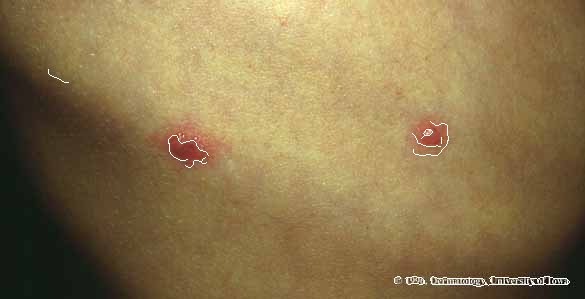
\includegraphics[scale=0.21]{Resources/Varicel-03_imagen_con_bordes.png} \\
	\column{1.5in}	
		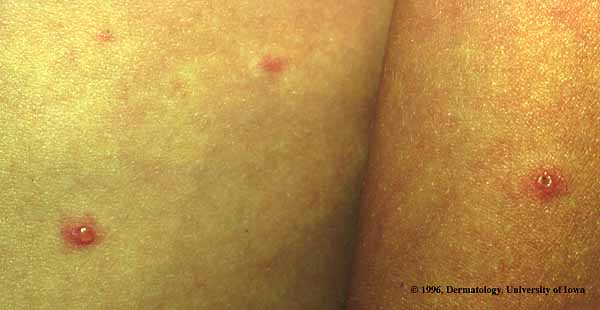
\includegraphics[scale=2.8]{Resources/Varicel-04.jpg} \\
		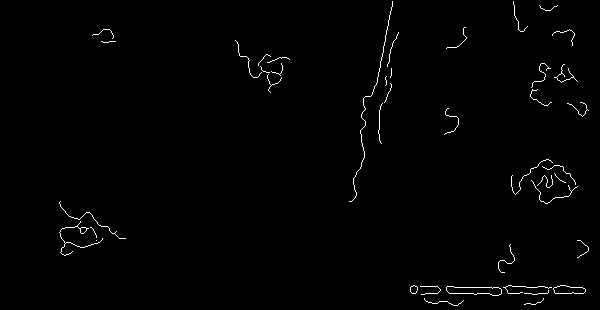
\includegraphics[scale=0.2]{Resources/Varicel-04_bordes_detectados.png} \\
		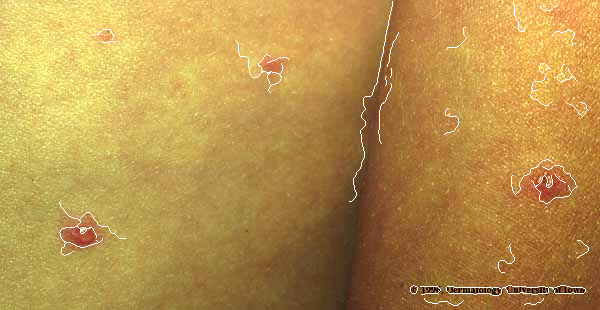
\includegraphics[scale=0.2]{Resources/Varicel-04_imagen_con_bordes.png} \\
	\end{columns}	
\end{frame}

\begin{frame}
	\frametitle{Ejemplo: Bordes detectados en la imagen}
	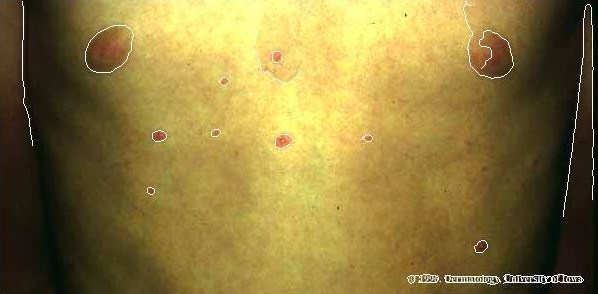
\includegraphics[width=4.3in]{Resources/bordesEnLaImagen-Varicel-01.jpg} \\
\end{frame}

\begin{frame}
	\frametitle{Ejemplo: Bordes detectados}
	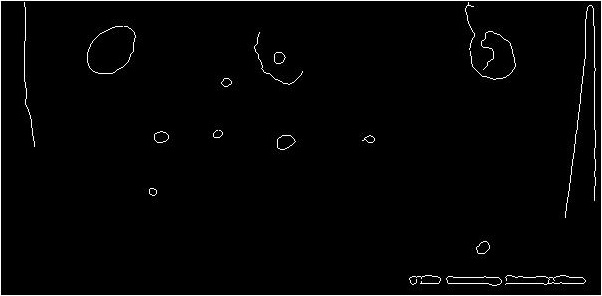
\includegraphics[width=4.3in]{Resources/bordes-Varicel-01.jpg}
\end{frame}

\subsection{Detecci�n de c�rculos}
\begin{frame}
	\frametitle{Detecci�n de c�rculos}
	\begin{itemize}
		\item �Dados los bordes, cu�ndo conforman un c�rculo?
		\item CHT: Circular Hough Transform
		\begin{itemize}
			\item Espacio de Hough
			\item Arreglo de acumulaci�n
		\end{itemize}
		\item Selecci�n de candidatos
		\begin{itemize}
			\item Ponderaci�n con respecto al m�ximo
			\item Umbralizaci�n
		\end{itemize}
	\end{itemize}
\end{frame}

\begin{frame}
	\frametitle{Ejemplo: Imagen con bordes detectados}
	\begin{figure}[h]
		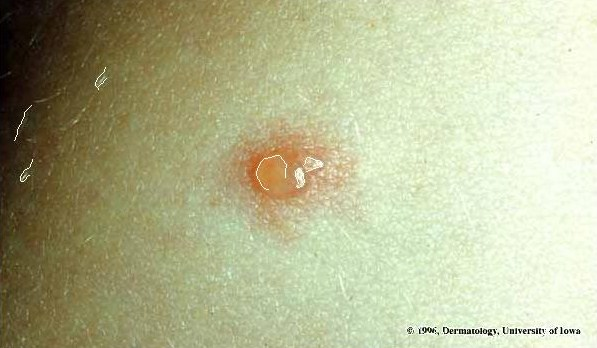
\includegraphics[width=4in]{Resources/resultado-Varicel-02-radio24-bordes.jpg}
	\end{figure}
\end{frame}

\begin{frame}
	\frametitle{Ejemplo: Arreglo de acumulaci�n}
	\begin{figure}[h]
		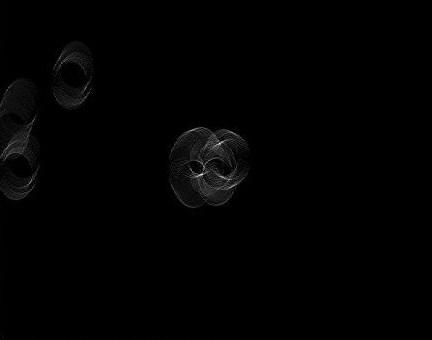
\includegraphics[width=3.5in]{Resources/acumulador-Varicel-02.jpg}
	\end{figure}
\end{frame}

\begin{frame}
	\frametitle{Ejemplo: Imagen con el c�rculo detectado}
	\begin{figure}[h]
		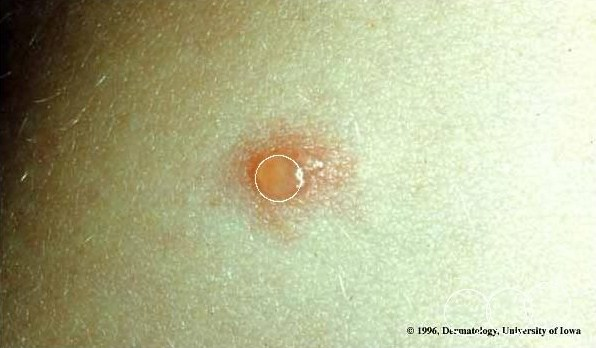
\includegraphics[width=4in]{Resources/resultado-Varicel-02-radio23_1.jpg}
	\end{figure}
\end{frame}

\subsection{Falsos positivos y falsos negativos}
\begin{frame}
	\frametitle{Falsos positivos y falsos negativos}
	\begin{itemize}
		\item Detecci�n de c�rculos redundantes
		\begin{figure}[h]
			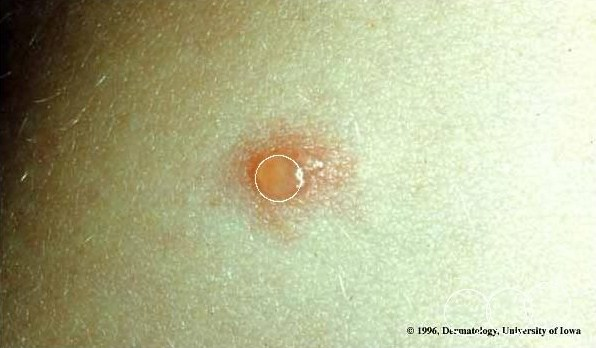
\includegraphics[width=2.2in]{Resources/resultado-Varicel-02-radio23_1.jpg}
			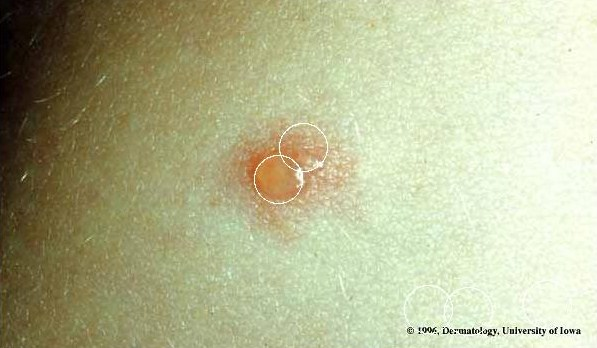
\includegraphics[width=2.2in]{Resources/resultado-Varicel-02-radio24.jpg}
		\end{figure}
		\item An�lisis del interior de la ampolla: Discriminaci�n
	\end{itemize}
\end{frame}
